
% Default to the notebook output style

    


% Inherit from the specified cell style.




    
\documentclass[11pt]{article}

    
    
    \usepackage[T1]{fontenc}
    % Nicer default font (+ math font) than Computer Modern for most use cases
    \usepackage{mathpazo}

    % Basic figure setup, for now with no caption control since it's done
    % automatically by Pandoc (which extracts ![](path) syntax from Markdown).
    \usepackage{graphicx}
    % We will generate all images so they have a width \maxwidth. This means
    % that they will get their normal width if they fit onto the page, but
    % are scaled down if they would overflow the margins.
    \makeatletter
    \def\maxwidth{\ifdim\Gin@nat@width>\linewidth\linewidth
    \else\Gin@nat@width\fi}
    \makeatother
    \let\Oldincludegraphics\includegraphics
    % Set max figure width to be 80% of text width, for now hardcoded.
    \renewcommand{\includegraphics}[1]{\Oldincludegraphics[width=.8\maxwidth]{#1}}
    % Ensure that by default, figures have no caption (until we provide a
    % proper Figure object with a Caption API and a way to capture that
    % in the conversion process - todo).
    \usepackage{caption}
    \DeclareCaptionLabelFormat{nolabel}{}
    \captionsetup{labelformat=nolabel}

    \usepackage{adjustbox} % Used to constrain images to a maximum size 
    \usepackage{xcolor} % Allow colors to be defined
    \usepackage{enumerate} % Needed for markdown enumerations to work
    \usepackage{geometry} % Used to adjust the document margins
    \usepackage{amsmath} % Equations
    \usepackage{amssymb} % Equations
    \usepackage{textcomp} % defines textquotesingle
    % Hack from http://tex.stackexchange.com/a/47451/13684:
    \AtBeginDocument{%
        \def\PYZsq{\textquotesingle}% Upright quotes in Pygmentized code
    }
    \usepackage{upquote} % Upright quotes for verbatim code
    \usepackage{eurosym} % defines \euro
    \usepackage[mathletters]{ucs} % Extended unicode (utf-8) support
    \usepackage[utf8x]{inputenc} % Allow utf-8 characters in the tex document
    \usepackage{fancyvrb} % verbatim replacement that allows latex
    \usepackage{grffile} % extends the file name processing of package graphics 
                         % to support a larger range 
    % The hyperref package gives us a pdf with properly built
    % internal navigation ('pdf bookmarks' for the table of contents,
    % internal cross-reference links, web links for URLs, etc.)
    \usepackage{hyperref}
    \usepackage{longtable} % longtable support required by pandoc >1.10
    \usepackage{booktabs}  % table support for pandoc > 1.12.2
    \usepackage[inline]{enumitem} % IRkernel/repr support (it uses the enumerate* environment)
    \usepackage[normalem]{ulem} % ulem is needed to support strikethroughs (\sout)
                                % normalem makes italics be italics, not underlines
    

    
    
    % Colors for the hyperref package
    \definecolor{urlcolor}{rgb}{0,.145,.698}
    \definecolor{linkcolor}{rgb}{.71,0.21,0.01}
    \definecolor{citecolor}{rgb}{.12,.54,.11}

    % ANSI colors
    \definecolor{ansi-black}{HTML}{3E424D}
    \definecolor{ansi-black-intense}{HTML}{282C36}
    \definecolor{ansi-red}{HTML}{E75C58}
    \definecolor{ansi-red-intense}{HTML}{B22B31}
    \definecolor{ansi-green}{HTML}{00A250}
    \definecolor{ansi-green-intense}{HTML}{007427}
    \definecolor{ansi-yellow}{HTML}{DDB62B}
    \definecolor{ansi-yellow-intense}{HTML}{B27D12}
    \definecolor{ansi-blue}{HTML}{208FFB}
    \definecolor{ansi-blue-intense}{HTML}{0065CA}
    \definecolor{ansi-magenta}{HTML}{D160C4}
    \definecolor{ansi-magenta-intense}{HTML}{A03196}
    \definecolor{ansi-cyan}{HTML}{60C6C8}
    \definecolor{ansi-cyan-intense}{HTML}{258F8F}
    \definecolor{ansi-white}{HTML}{C5C1B4}
    \definecolor{ansi-white-intense}{HTML}{A1A6B2}

    % commands and environments needed by pandoc snippets
    % extracted from the output of `pandoc -s`
    \providecommand{\tightlist}{%
      \setlength{\itemsep}{0pt}\setlength{\parskip}{0pt}}
    \DefineVerbatimEnvironment{Highlighting}{Verbatim}{commandchars=\\\{\}}
    % Add ',fontsize=\small' for more characters per line
    \newenvironment{Shaded}{}{}
    \newcommand{\KeywordTok}[1]{\textcolor[rgb]{0.00,0.44,0.13}{\textbf{{#1}}}}
    \newcommand{\DataTypeTok}[1]{\textcolor[rgb]{0.56,0.13,0.00}{{#1}}}
    \newcommand{\DecValTok}[1]{\textcolor[rgb]{0.25,0.63,0.44}{{#1}}}
    \newcommand{\BaseNTok}[1]{\textcolor[rgb]{0.25,0.63,0.44}{{#1}}}
    \newcommand{\FloatTok}[1]{\textcolor[rgb]{0.25,0.63,0.44}{{#1}}}
    \newcommand{\CharTok}[1]{\textcolor[rgb]{0.25,0.44,0.63}{{#1}}}
    \newcommand{\StringTok}[1]{\textcolor[rgb]{0.25,0.44,0.63}{{#1}}}
    \newcommand{\CommentTok}[1]{\textcolor[rgb]{0.38,0.63,0.69}{\textit{{#1}}}}
    \newcommand{\OtherTok}[1]{\textcolor[rgb]{0.00,0.44,0.13}{{#1}}}
    \newcommand{\AlertTok}[1]{\textcolor[rgb]{1.00,0.00,0.00}{\textbf{{#1}}}}
    \newcommand{\FunctionTok}[1]{\textcolor[rgb]{0.02,0.16,0.49}{{#1}}}
    \newcommand{\RegionMarkerTok}[1]{{#1}}
    \newcommand{\ErrorTok}[1]{\textcolor[rgb]{1.00,0.00,0.00}{\textbf{{#1}}}}
    \newcommand{\NormalTok}[1]{{#1}}
    
    % Additional commands for more recent versions of Pandoc
    \newcommand{\ConstantTok}[1]{\textcolor[rgb]{0.53,0.00,0.00}{{#1}}}
    \newcommand{\SpecialCharTok}[1]{\textcolor[rgb]{0.25,0.44,0.63}{{#1}}}
    \newcommand{\VerbatimStringTok}[1]{\textcolor[rgb]{0.25,0.44,0.63}{{#1}}}
    \newcommand{\SpecialStringTok}[1]{\textcolor[rgb]{0.73,0.40,0.53}{{#1}}}
    \newcommand{\ImportTok}[1]{{#1}}
    \newcommand{\DocumentationTok}[1]{\textcolor[rgb]{0.73,0.13,0.13}{\textit{{#1}}}}
    \newcommand{\AnnotationTok}[1]{\textcolor[rgb]{0.38,0.63,0.69}{\textbf{\textit{{#1}}}}}
    \newcommand{\CommentVarTok}[1]{\textcolor[rgb]{0.38,0.63,0.69}{\textbf{\textit{{#1}}}}}
    \newcommand{\VariableTok}[1]{\textcolor[rgb]{0.10,0.09,0.49}{{#1}}}
    \newcommand{\ControlFlowTok}[1]{\textcolor[rgb]{0.00,0.44,0.13}{\textbf{{#1}}}}
    \newcommand{\OperatorTok}[1]{\textcolor[rgb]{0.40,0.40,0.40}{{#1}}}
    \newcommand{\BuiltInTok}[1]{{#1}}
    \newcommand{\ExtensionTok}[1]{{#1}}
    \newcommand{\PreprocessorTok}[1]{\textcolor[rgb]{0.74,0.48,0.00}{{#1}}}
    \newcommand{\AttributeTok}[1]{\textcolor[rgb]{0.49,0.56,0.16}{{#1}}}
    \newcommand{\InformationTok}[1]{\textcolor[rgb]{0.38,0.63,0.69}{\textbf{\textit{{#1}}}}}
    \newcommand{\WarningTok}[1]{\textcolor[rgb]{0.38,0.63,0.69}{\textbf{\textit{{#1}}}}}
    
    
    % Define a nice break command that doesn't care if a line doesn't already
    % exist.
    \def\br{\hspace*{\fill} \\* }
    % Math Jax compatability definitions
    \def\gt{>}
    \def\lt{<}
    % Document parameters
    \title{STA663-Final-Report}
    
    
    

    % Pygments definitions
    
\makeatletter
\def\PY@reset{\let\PY@it=\relax \let\PY@bf=\relax%
    \let\PY@ul=\relax \let\PY@tc=\relax%
    \let\PY@bc=\relax \let\PY@ff=\relax}
\def\PY@tok#1{\csname PY@tok@#1\endcsname}
\def\PY@toks#1+{\ifx\relax#1\empty\else%
    \PY@tok{#1}\expandafter\PY@toks\fi}
\def\PY@do#1{\PY@bc{\PY@tc{\PY@ul{%
    \PY@it{\PY@bf{\PY@ff{#1}}}}}}}
\def\PY#1#2{\PY@reset\PY@toks#1+\relax+\PY@do{#2}}

\expandafter\def\csname PY@tok@w\endcsname{\def\PY@tc##1{\textcolor[rgb]{0.73,0.73,0.73}{##1}}}
\expandafter\def\csname PY@tok@c\endcsname{\let\PY@it=\textit\def\PY@tc##1{\textcolor[rgb]{0.25,0.50,0.50}{##1}}}
\expandafter\def\csname PY@tok@cp\endcsname{\def\PY@tc##1{\textcolor[rgb]{0.74,0.48,0.00}{##1}}}
\expandafter\def\csname PY@tok@k\endcsname{\let\PY@bf=\textbf\def\PY@tc##1{\textcolor[rgb]{0.00,0.50,0.00}{##1}}}
\expandafter\def\csname PY@tok@kp\endcsname{\def\PY@tc##1{\textcolor[rgb]{0.00,0.50,0.00}{##1}}}
\expandafter\def\csname PY@tok@kt\endcsname{\def\PY@tc##1{\textcolor[rgb]{0.69,0.00,0.25}{##1}}}
\expandafter\def\csname PY@tok@o\endcsname{\def\PY@tc##1{\textcolor[rgb]{0.40,0.40,0.40}{##1}}}
\expandafter\def\csname PY@tok@ow\endcsname{\let\PY@bf=\textbf\def\PY@tc##1{\textcolor[rgb]{0.67,0.13,1.00}{##1}}}
\expandafter\def\csname PY@tok@nb\endcsname{\def\PY@tc##1{\textcolor[rgb]{0.00,0.50,0.00}{##1}}}
\expandafter\def\csname PY@tok@nf\endcsname{\def\PY@tc##1{\textcolor[rgb]{0.00,0.00,1.00}{##1}}}
\expandafter\def\csname PY@tok@nc\endcsname{\let\PY@bf=\textbf\def\PY@tc##1{\textcolor[rgb]{0.00,0.00,1.00}{##1}}}
\expandafter\def\csname PY@tok@nn\endcsname{\let\PY@bf=\textbf\def\PY@tc##1{\textcolor[rgb]{0.00,0.00,1.00}{##1}}}
\expandafter\def\csname PY@tok@ne\endcsname{\let\PY@bf=\textbf\def\PY@tc##1{\textcolor[rgb]{0.82,0.25,0.23}{##1}}}
\expandafter\def\csname PY@tok@nv\endcsname{\def\PY@tc##1{\textcolor[rgb]{0.10,0.09,0.49}{##1}}}
\expandafter\def\csname PY@tok@no\endcsname{\def\PY@tc##1{\textcolor[rgb]{0.53,0.00,0.00}{##1}}}
\expandafter\def\csname PY@tok@nl\endcsname{\def\PY@tc##1{\textcolor[rgb]{0.63,0.63,0.00}{##1}}}
\expandafter\def\csname PY@tok@ni\endcsname{\let\PY@bf=\textbf\def\PY@tc##1{\textcolor[rgb]{0.60,0.60,0.60}{##1}}}
\expandafter\def\csname PY@tok@na\endcsname{\def\PY@tc##1{\textcolor[rgb]{0.49,0.56,0.16}{##1}}}
\expandafter\def\csname PY@tok@nt\endcsname{\let\PY@bf=\textbf\def\PY@tc##1{\textcolor[rgb]{0.00,0.50,0.00}{##1}}}
\expandafter\def\csname PY@tok@nd\endcsname{\def\PY@tc##1{\textcolor[rgb]{0.67,0.13,1.00}{##1}}}
\expandafter\def\csname PY@tok@s\endcsname{\def\PY@tc##1{\textcolor[rgb]{0.73,0.13,0.13}{##1}}}
\expandafter\def\csname PY@tok@sd\endcsname{\let\PY@it=\textit\def\PY@tc##1{\textcolor[rgb]{0.73,0.13,0.13}{##1}}}
\expandafter\def\csname PY@tok@si\endcsname{\let\PY@bf=\textbf\def\PY@tc##1{\textcolor[rgb]{0.73,0.40,0.53}{##1}}}
\expandafter\def\csname PY@tok@se\endcsname{\let\PY@bf=\textbf\def\PY@tc##1{\textcolor[rgb]{0.73,0.40,0.13}{##1}}}
\expandafter\def\csname PY@tok@sr\endcsname{\def\PY@tc##1{\textcolor[rgb]{0.73,0.40,0.53}{##1}}}
\expandafter\def\csname PY@tok@ss\endcsname{\def\PY@tc##1{\textcolor[rgb]{0.10,0.09,0.49}{##1}}}
\expandafter\def\csname PY@tok@sx\endcsname{\def\PY@tc##1{\textcolor[rgb]{0.00,0.50,0.00}{##1}}}
\expandafter\def\csname PY@tok@m\endcsname{\def\PY@tc##1{\textcolor[rgb]{0.40,0.40,0.40}{##1}}}
\expandafter\def\csname PY@tok@gh\endcsname{\let\PY@bf=\textbf\def\PY@tc##1{\textcolor[rgb]{0.00,0.00,0.50}{##1}}}
\expandafter\def\csname PY@tok@gu\endcsname{\let\PY@bf=\textbf\def\PY@tc##1{\textcolor[rgb]{0.50,0.00,0.50}{##1}}}
\expandafter\def\csname PY@tok@gd\endcsname{\def\PY@tc##1{\textcolor[rgb]{0.63,0.00,0.00}{##1}}}
\expandafter\def\csname PY@tok@gi\endcsname{\def\PY@tc##1{\textcolor[rgb]{0.00,0.63,0.00}{##1}}}
\expandafter\def\csname PY@tok@gr\endcsname{\def\PY@tc##1{\textcolor[rgb]{1.00,0.00,0.00}{##1}}}
\expandafter\def\csname PY@tok@ge\endcsname{\let\PY@it=\textit}
\expandafter\def\csname PY@tok@gs\endcsname{\let\PY@bf=\textbf}
\expandafter\def\csname PY@tok@gp\endcsname{\let\PY@bf=\textbf\def\PY@tc##1{\textcolor[rgb]{0.00,0.00,0.50}{##1}}}
\expandafter\def\csname PY@tok@go\endcsname{\def\PY@tc##1{\textcolor[rgb]{0.53,0.53,0.53}{##1}}}
\expandafter\def\csname PY@tok@gt\endcsname{\def\PY@tc##1{\textcolor[rgb]{0.00,0.27,0.87}{##1}}}
\expandafter\def\csname PY@tok@err\endcsname{\def\PY@bc##1{\setlength{\fboxsep}{0pt}\fcolorbox[rgb]{1.00,0.00,0.00}{1,1,1}{\strut ##1}}}
\expandafter\def\csname PY@tok@kc\endcsname{\let\PY@bf=\textbf\def\PY@tc##1{\textcolor[rgb]{0.00,0.50,0.00}{##1}}}
\expandafter\def\csname PY@tok@kd\endcsname{\let\PY@bf=\textbf\def\PY@tc##1{\textcolor[rgb]{0.00,0.50,0.00}{##1}}}
\expandafter\def\csname PY@tok@kn\endcsname{\let\PY@bf=\textbf\def\PY@tc##1{\textcolor[rgb]{0.00,0.50,0.00}{##1}}}
\expandafter\def\csname PY@tok@kr\endcsname{\let\PY@bf=\textbf\def\PY@tc##1{\textcolor[rgb]{0.00,0.50,0.00}{##1}}}
\expandafter\def\csname PY@tok@bp\endcsname{\def\PY@tc##1{\textcolor[rgb]{0.00,0.50,0.00}{##1}}}
\expandafter\def\csname PY@tok@fm\endcsname{\def\PY@tc##1{\textcolor[rgb]{0.00,0.00,1.00}{##1}}}
\expandafter\def\csname PY@tok@vc\endcsname{\def\PY@tc##1{\textcolor[rgb]{0.10,0.09,0.49}{##1}}}
\expandafter\def\csname PY@tok@vg\endcsname{\def\PY@tc##1{\textcolor[rgb]{0.10,0.09,0.49}{##1}}}
\expandafter\def\csname PY@tok@vi\endcsname{\def\PY@tc##1{\textcolor[rgb]{0.10,0.09,0.49}{##1}}}
\expandafter\def\csname PY@tok@vm\endcsname{\def\PY@tc##1{\textcolor[rgb]{0.10,0.09,0.49}{##1}}}
\expandafter\def\csname PY@tok@sa\endcsname{\def\PY@tc##1{\textcolor[rgb]{0.73,0.13,0.13}{##1}}}
\expandafter\def\csname PY@tok@sb\endcsname{\def\PY@tc##1{\textcolor[rgb]{0.73,0.13,0.13}{##1}}}
\expandafter\def\csname PY@tok@sc\endcsname{\def\PY@tc##1{\textcolor[rgb]{0.73,0.13,0.13}{##1}}}
\expandafter\def\csname PY@tok@dl\endcsname{\def\PY@tc##1{\textcolor[rgb]{0.73,0.13,0.13}{##1}}}
\expandafter\def\csname PY@tok@s2\endcsname{\def\PY@tc##1{\textcolor[rgb]{0.73,0.13,0.13}{##1}}}
\expandafter\def\csname PY@tok@sh\endcsname{\def\PY@tc##1{\textcolor[rgb]{0.73,0.13,0.13}{##1}}}
\expandafter\def\csname PY@tok@s1\endcsname{\def\PY@tc##1{\textcolor[rgb]{0.73,0.13,0.13}{##1}}}
\expandafter\def\csname PY@tok@mb\endcsname{\def\PY@tc##1{\textcolor[rgb]{0.40,0.40,0.40}{##1}}}
\expandafter\def\csname PY@tok@mf\endcsname{\def\PY@tc##1{\textcolor[rgb]{0.40,0.40,0.40}{##1}}}
\expandafter\def\csname PY@tok@mh\endcsname{\def\PY@tc##1{\textcolor[rgb]{0.40,0.40,0.40}{##1}}}
\expandafter\def\csname PY@tok@mi\endcsname{\def\PY@tc##1{\textcolor[rgb]{0.40,0.40,0.40}{##1}}}
\expandafter\def\csname PY@tok@il\endcsname{\def\PY@tc##1{\textcolor[rgb]{0.40,0.40,0.40}{##1}}}
\expandafter\def\csname PY@tok@mo\endcsname{\def\PY@tc##1{\textcolor[rgb]{0.40,0.40,0.40}{##1}}}
\expandafter\def\csname PY@tok@ch\endcsname{\let\PY@it=\textit\def\PY@tc##1{\textcolor[rgb]{0.25,0.50,0.50}{##1}}}
\expandafter\def\csname PY@tok@cm\endcsname{\let\PY@it=\textit\def\PY@tc##1{\textcolor[rgb]{0.25,0.50,0.50}{##1}}}
\expandafter\def\csname PY@tok@cpf\endcsname{\let\PY@it=\textit\def\PY@tc##1{\textcolor[rgb]{0.25,0.50,0.50}{##1}}}
\expandafter\def\csname PY@tok@c1\endcsname{\let\PY@it=\textit\def\PY@tc##1{\textcolor[rgb]{0.25,0.50,0.50}{##1}}}
\expandafter\def\csname PY@tok@cs\endcsname{\let\PY@it=\textit\def\PY@tc##1{\textcolor[rgb]{0.25,0.50,0.50}{##1}}}

\def\PYZbs{\char`\\}
\def\PYZus{\char`\_}
\def\PYZob{\char`\{}
\def\PYZcb{\char`\}}
\def\PYZca{\char`\^}
\def\PYZam{\char`\&}
\def\PYZlt{\char`\<}
\def\PYZgt{\char`\>}
\def\PYZsh{\char`\#}
\def\PYZpc{\char`\%}
\def\PYZdl{\char`\$}
\def\PYZhy{\char`\-}
\def\PYZsq{\char`\'}
\def\PYZdq{\char`\"}
\def\PYZti{\char`\~}
% for compatibility with earlier versions
\def\PYZat{@}
\def\PYZlb{[}
\def\PYZrb{]}
\makeatother


    % Exact colors from NB
    \definecolor{incolor}{rgb}{0.0, 0.0, 0.5}
    \definecolor{outcolor}{rgb}{0.545, 0.0, 0.0}



    
    % Prevent overflowing lines due to hard-to-break entities
    \sloppy 
    % Setup hyperref package
    \hypersetup{
      breaklinks=true,  % so long urls are correctly broken across lines
      colorlinks=true,
      urlcolor=urlcolor,
      linkcolor=linkcolor,
      citecolor=citecolor,
      }
    % Slightly bigger margins than the latex defaults
    
    \geometry{verbose,tmargin=1in,bmargin=1in,lmargin=1in,rmargin=1in}
    
    

    \begin{document}
    
    
    \maketitle
    
    

    
    \hypertarget{implementation-of-indian-buffet-process-prior-in-an-infinite-latent-feature-model}{%
\section{Implementation of Indian Buffet Process Prior in an Infinite
Latent Feature
Model}\label{implementation-of-indian-buffet-process-prior-in-an-infinite-latent-feature-model}}

\hypertarget{by-xiaohe-yang-zhi-qiu}{%
\subsection{By Xiaohe Yang \& Zhi Qiu}\label{by-xiaohe-yang-zhi-qiu}}

    \hypertarget{abstract}{%
\subsubsection{Abstract}\label{abstract}}

    \hypertarget{background}{%
\subsubsection{Background}\label{background}}

    In latent class models such as finite mixture models, observed data
points are realizations from some distribution determined by a single
class {[}2{]}. Usually, the number of such classes has to be chosen and
fixed. Infinite Dirichlet process mixture models with priors like
Chinese Reataurant Process (CRP) break this limitation by allowing an
infinite number of latent classes and allow clustering with a
potentially infinite number of clusters. However, each point is still
limited to one cluster and in real world settings data points are very
likely to share multiple classes. For instance, in the problem of
clustering instances of human beings appearing in different contexts
across a set of images, all such instances to share a cluster for human
to different degrees depending on the context in which they appear
{[}2{]}. Therefore, latent feature models are used to model these
problems where data points share multiple clusters. Similar to the
latent class cases, for finite latent feature models the number of
features is finite and has to be specified a priori, while in infinite
latent feature models such a pre-selecting the number of features could
be avoided. Specifically, Indian Buffet Process (IBP) is a quite popular
prior distribution that could be used in an infinite latent feature
model {[}1{]}.

There are many sampling models that could be used together with IBP to
conduct infinite latent feature modelling. In this paper we will mainly
focus on the Gaussian sampling distribution and explore IBP's
application in an infinite binary linear-Gaussian latent feature model.

    \hypertarget{algorithm-description}{%
\subsubsection{Algorithm Description}\label{algorithm-description}}

    \hypertarget{indian-buffet-process}{%
\paragraph{- Indian Buffet Process}\label{indian-buffet-process}}

Firstly, IBP is a stochastic process for defining the probability
distribution over equivalence classes of sparse binary matrices with a
finite number of rows and an unbounded number of columns {[}6{]}. It is
a metaphor of Indian restaurants offering buffets with a
close-to-infinite number of dishes, and the number of dishes (latent
features) chosen by a customer follows a Poisson distribution {[}3{]}.

The detailed procedure is as the following: N customers enter a
restaurant one after another. The first customer starts at the left of
the buffet and takes a serving from each dish, stopping after a
Poisson(\(\alpha\)) number of dishes. The \(i\)th customer moves along
the buffet, sampling dishes in proportion to their popularity (thus
customers/obervations are not independent of each other, but note that
the dishes/latent features are independent), taking dish \(k\) with
probability \(\frac{m_k}{i}\) , where \(m_k\) is the number of previous
customers who have sampled that dish. Having reached the end of all
previous sampled dishes, the \(i\)th customer then tries a
Poisson(\(\frac{\alpha}{i}\)) number of new dishes. Customer choice of
dishes is indicated using a binary matrix \(Z\) with \(N\) rows and
infinitely many columns(corresponding to the infinitely many selection
of dishes), where \(z_{ik} = 1\) if the \(i\)th costumer sampled the
\(k\)th dish {[}1{]}.

Mathematically, the probability of a binary matrix,
\(Z \sim IBP(\alpha)\) is given by

\[P(Z| \alpha) = \frac{\alpha^{K}}{\prod_{h=1}^{2^N - 1} K_{h}!} exp \{ - \alpha H_{N}\} \prod_{k=1}^{K} \frac{(N- m_k)! (m_k - 1)!}{N!}\]

\(N\) - Number of objects/obeservations

\(K\) - Total number of latent features

\(K_h\) - Number of features with history h (whether the \(N\) objects
possess this feature)

\(H_N = \sum_{k=1}^{N} \frac{1}{k}\) - the \(N^{th}\) harmonic number

\(m_k\) - Number of objects with feature k

\(\alpha\) - parameter influencing the Indian Buffet Process's number of
features

A detailed derivation of the equation can be found in Griffiths \&
Ghahramani, 2005 {[}1{]}.

The conditional distribution in IBP (which is the infinite case) is be
given by

\[ P( z_{i,k} = 1 \mid z_{-i,k}) = \frac{m_{-i, k}}{N}\]

where \(z_{−i,k}\) is the assignment of feature k for all objects except
the \(i\)th object and \(m_{−i,k}\) is the number of objects with
feature k except the \(i\)th object.

    Then, we use IBP as a prior and combine it with a Linear Gaussian
sampling model to do Gibbs sampling/ Metropolis Hastings for an infinite
binary linear-Gaussian latent feature model.

    \hypertarget{linear-gaussian-binary-latent-feature-model}{%
\paragraph{- Linear-Gaussian Binary Latent Feature
Model}\label{linear-gaussian-binary-latent-feature-model}}

The mathematical set-up is as the following:

\(Z\) - a binary feature ownership matrix (indicator matrix), where
\(z_{i,k}=1\) indicating that object \(i\) posssess latent feature \(k\)

\(Z \sim IBP(\alpha)\)

\(X\) - real-valued observation matrix, where \(x_{i,j}\) is the value
of feature \(j\) for object \(i\), a \({N x D}\) matrix

\[x_i \sim \text{Normal}(z_i A, \sigma_X^2 I) \]

\(A\) - a \({K x D}\) matrix of weights representing the \(\textit{K}\)
latent features.

\[A \sim \text{Normal}(0, \sigma_A^2 I)\]

The likelihood is (after marginalizing out \(A\)):

\[P(X|Z,\sigma_X, \sigma_A) = \frac{1}{(2 \pi)^{ND/2} (\sigma_X)^{(N-K)D}(\sigma_A)^{KD}(|Z^TZ+\frac{\sigma_X^2}{\sigma_A^2}I|)^{D/2}} exp\{-\frac{1}{2\sigma_X^2}tr(X^T(I-Z M Z^T)X)\}\]

where \[ M = (Z^TZ+\frac{\sigma_X^2}{\sigma_A^2}I)^{-1}\]

    \hypertarget{monte-carlo-simulation-structure}{%
\paragraph{- Monte Carlo Simulation
Structure}\label{monte-carlo-simulation-structure}}

We have five parameters of interest in this model that need to be
updated throughout the MCMC process.

1.) Z: feature ownernship matrix

2.) \(K_+\): number of new latent features

3.) \(\alpha\): parameter controlling \(K_+\)

4.) \(\sigma_X\)

5.) \(\sigma_A\)

There are full conditional distributions for Z, \(K_+\), and \(\alpha\),
so can use Gibbs Sampling (a special case of Metropolis Hastings). AS
for \(\sigma_X\) and \(\sigma_A\), the general Metropolis-Hastings
algorithm is applied.

Priors:

\[P(z_{ik} = 1 | \textbf{z}_{-i,k}) = \dfrac{m_{-i,k}}{N} \]

\[\alpha \sim \text{Gamma}(1,1)\]

\[K_+ \sim \text{Poisson}(\dfrac{\alpha}{N})\]

Gibbs Sampling Updates:

\begin{enumerate}
\def\labelenumi{\arabic{enumi}.}
\tightlist
\item
  For observation \(i\) with more than one feature, sample \(z_{i,k}\)
  using the full conditional distribution.
\end{enumerate}

\[P(z_{ik}|X,Z_{-(i,k),},\sigma_X,\sigma_A) \propto  P(X|Z,\sigma_X, \sigma_A) * P(z_{ik}=1|\textbf{z}_{-i,k})\]

\begin{enumerate}
\def\labelenumi{\arabic{enumi}.}
\setcounter{enumi}{1}
\item
  Sample new features for observation \(i\) by first computing a
  truncated distribution for \(K_+\) using the data likelihood and the
  prior for \(K_+\) up to 4 new features, and then sampling from the
  truncated distribution.
\item
  Sample
  \(P(\alpha \mid Z) \sim Gamma(1 + K_+, 1 + \sum_{i=1}^{N} H_i)\)
\end{enumerate}

Metropolis-Hasting Updates:

Update \(\sigma_X\) and \(\sigma_A\) using Metropolis-Hastings. For
\(\sigma_X\), generate a random value from a Uniform(-.05, .05)
distribution and add this value to our current value of \(\sigma_X\) to
get \(\sigma_X^*\). Accept new value of \(\sigma_X\) with probability:

\[p = min(1, \dfrac{P(X|Z, \sigma_X^*, \sigma_A}{P(X|Z, \sigma_X, \sigma_A})\]

To update \(\sigma_A\), follow the same proceedure as with \(\sigma_X\),
replacing \(\sigma_X\) with \(\sigma_A\).

    \hypertarget{optimization}{%
\subsubsection{Optimization}\label{optimization}}

    \begin{itemize}
\tightlist
\item
  Algorithm:
\end{itemize}

    After profiling (output result is stored in Original\_Algorithm.ipynb),
the likelihood function part is what takes the most of computation time.
To reduce the number of calls and speed up sampling, the organization of
the sampling functions is modified: the calculation of the M matrix is
moved into the likelihood function.

As is shown in the time comparison table for likelihood table in
Optimized\_Algorithm.ipynb, there is an obvious improvement in time
(from 0.000451 to 0.000307) with the new likelihood function. Moreover,
as shown in the time comparison table for overall MCMC samling, the
optimized algorithm improved from a time of 46.409353 to 41.323922,
which is a 10.96\% improvement.

    \begin{itemize}
\tightlist
\item
  Cython
\end{itemize}

    As for Cython, after writing the MCMC algorithm in C style, the the time
comparison table result in Optimized\_Cython shows that the time for our
original algorithm is 58.640440 while the time of running for the Cython
version is 48.795563, which is a 16.79\% improvement.

    \hypertarget{application-to-simulated-data-and-real-data}{%
\subsubsection{Application to Simulated Data and Real
Data}\label{application-to-simulated-data-and-real-data}}

    For a demonstration of the algorithim, we simulated image data as
proposed by Yildrim {[}7{]}. Four base images were created consisting of
\(6x6\) pixels. Thus, each image can be represented by a vector of
length 36. The latent features can be represented by a \(KxD\) weight
matrix A where \(K=4\) and \(D=36\). \(X\) is an \(N × D\) matrix that
represents the images generated by the \(K\) bases (each basis is
present with probability 0.5 and \(N=100\)).

    The four base (latent) images are shown below:

    \begin{figure}
\centering
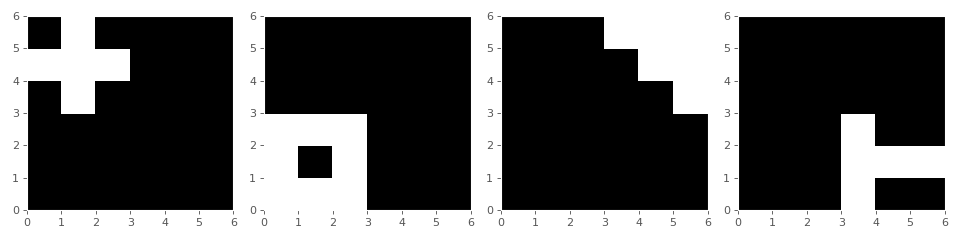
\includegraphics{basis_images.png}
\caption{Latent Feature Matrices}
\end{figure}

    The four bases altogether formulates the latent feature matrices A, then
100 synthetic images are created via simulation, where each image
\(x_i\) is a superposition of zero or more base images (latent features)
with added white noise. \(X\) is a \(100 x D\) matrix. Here, \(z_i\) is
a row of a binary feature matrix \(Z\) of dimension \(100 x K\). A
values in \(z_i\) is 1 or 0 with a probability of 0.5. A value of 1 in
\(z_i\) corresponds to image \(x_i\) containing the correspoing base
image. \(\sigma_x^2\), which controls the white noise, is set to 0.5.

An example image of the simulated dataset which is generated by our
sampling algorithm is shown as below:

    \begin{figure}
\centering
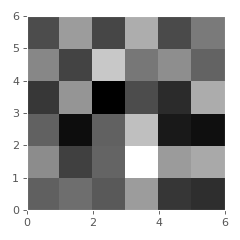
\includegraphics{simulated_images.png}
\caption{Latent Feature Matrices}
\end{figure}

    As for the MCMC results from a simulted data set, we represent them by
presenting traceplots of the parameters \(K, \sigma_X, \sigma_A\) and
\(\alpha\). It is shown in the above traceplots that the convergence of
our Markov chain is good and \(\sigma_X\) converges to its true value
0.5:

    \begin{figure}
\centering
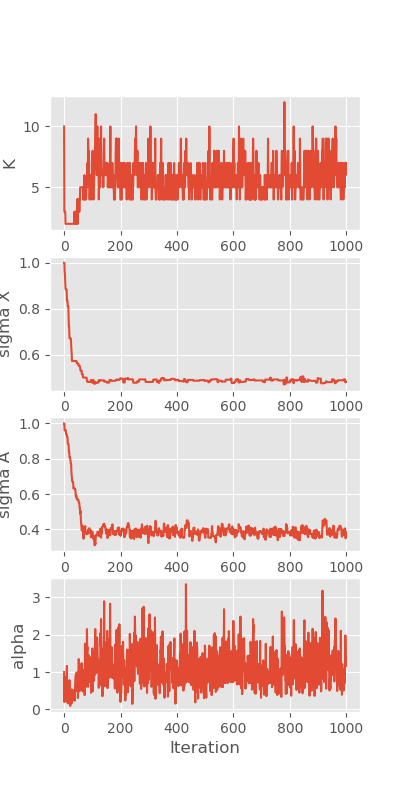
\includegraphics{traceplots_simulation.png}
\caption{traceplots}
\end{figure}

    \hypertarget{comparison-with-competing-algorithms}{%
\subsubsection{Comparison with Competing
Algorithms}\label{comparison-with-competing-algorithms}}

    \hypertarget{conclusion}{%
\subsubsection{Conclusion}\label{conclusion}}

    \hypertarget{references}{%
\subsubsection{References}\label{references}}

{[}1{]} Thomas L. Griffiths and Zoubin Ghahramani. Infinite latent
feature models and the Indian buffet process. 2005.

{[}2{]} Eric P. Xing. 21: The Indian Buffet Process {[}Lecture{]}. 2014

{[}3{]} Christine Chai. Implementation of the Indian Buffet Process.
2015.

{[}4{]} Dipesh Gautam. Indian Buffet Process and its application in the
Infinite Latent Feature Model. 2015.

{[}5{]} Radhika Anand. Infinite Latent Feature Models and the Indian
Buffet Process. 2015.

{[}6{]} Drew Jordan and Sunith Suresh. The Indian Buffet Process and
Applications for Unsupervised Learning. 2016.

{[}7{]} Ilker Yildirim. Bayesian statistics: Indian buffet process.
2012.


    % Add a bibliography block to the postdoc
    
    
    
    \end{document}
